\begin{statementbox}
  \textbf{\textcolor{CStatement}{它解决什么问题？}}
  已知 $y=f(x)$ 的图像，想让它\textbf{横向变窄或变宽}，却保持每个点的高度不变，应该怎样改解析式？

  \medskip
  \textbf{\textcolor{CStatement}{核心结论：横坐标乘 $k$，括号里的 $x$ 就除以 $k$}}
  \begin{description}[style=nextline, leftmargin=2.8em, labelsep=0.5em, itemsep=0.4em]
    \item[\textbf{条件：}] 原函数为 $y=f(x)$；所有点的\textbf{横坐标变为原来的 $k$ 倍}（$k>0$），\textbf{纵坐标不变}。
    \item[\textbf{新解析式：}]
      \[
        \boxed{\ y=f\!\left(\frac{x}{k}\right)\ }
      \]
    \item[\textbf{另一种写法：}] 若新函数写成 $y=f(\omega x)$（$\omega>0$），那么横坐标实际变为原来的 $\dfrac{1}{\omega}$，即 $k=\dfrac{1}{\omega}$。
  \end{description}

  \begin{center}
  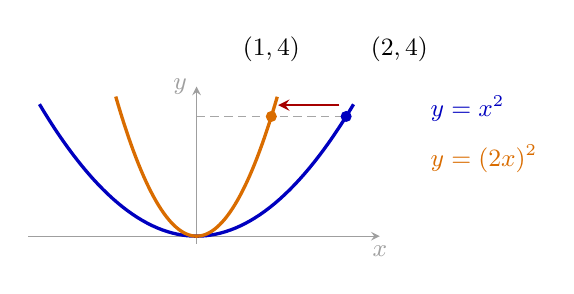
\begin{tikzpicture}[x=0.95cm,y=0.38cm,>=stealth,every node/.style={font=\small}]
    \draw[->,gray!75] (-2.25,0)--(2.45,0) node[below] {$x$};
    \draw[->,gray!75] (0,-0.25)--(0,5.0) node[left] {$y$};
    \draw[very thick,blue!75!black,domain=-2.1:2.1,samples=65] plot (\x,{\x*\x});
    \draw[very thick,orange!85!black,domain=-1.08:1.08,samples=65] plot (\x,{4*\x*\x});
    \draw[densely dashed,gray!70] (0,4)--(2.05,4);
    \fill[blue!75!black] (2,4) circle (2pt);
    \fill[orange!85!black] (1,4) circle (2pt);
    \draw[->,thick,red!65!black] (1.91,4.38)--(1.09,4.38);
    \node[above right,blue!75!black] at (3,3.5) {$y=x^2$};
    \node[above right,orange!85!black] at (3,1.8) {$y=(2x)^2$};
    \node[above right] at (2.2,5.5) {$(2,4)$};
    \node[above] at (1,5.5) {$(1,4)$};
  \end{tikzpicture}

  \end{center}
  \noindent\textbf{看图记住：} $(2,4)\to(1,4)$，高度都是 $4$，横坐标减半；所以 $f(2x)$ \textbf{变窄}，不是变宽。

  \medskip
  \textbf{\textcolor{CStatement}{一眼判断}}
  \begin{itemize}[leftmargin=*,itemsep=0.2em,topsep=0.2em]
    \item $\omega>1$：$f(\omega x)$ 横向\textbf{压缩}到 $1/\omega$；
    \item $0<\omega<1$：$f(\omega x)$ 横向\textbf{拉伸}到 $1/\omega$；
    \item $\omega=1$（或 $k=1$）：图像\textbf{不变}。
  \end{itemize}
\end{statementbox}
